%----------------------------------------------------------------------------------------
%  A1 portrait poster: Implementing Conditional Access on FPGA
%  Compile with pdfLaTeX (Overleaf). Replace every [PLACEHOLDER]; upload logo.png.
%
%  Layout: two balanced columns, verified locally to fit one A1 page. If you add text
%  and it spills onto page 2, lower \figscale or a figure width.
%----------------------------------------------------------------------------------------

\documentclass{article}
\usepackage[paperwidth=594mm,paperheight=841mm,margin=10mm]{geometry}

\usepackage[T1]{fontenc}
\usepackage{newtxtext,newtxmath}   % Times
\usepackage{newtxtt}               % matching typewriter face for code
\usepackage{anyfontsize}

\usepackage[dvipsnames]{xcolor}
\definecolor{navy}{HTML}{1F3A5F}
\definecolor{rulegray}{HTML}{B5B5B5}
\definecolor{captiongray}{HTML}{333333}

\usepackage{multicol}
\setlength{\columnsep}{12mm}
\setlength{\columnseprule}{0.6pt}
\renewcommand{\columnseprulecolor}{\color{rulegray}}

\usepackage{graphicx}
\graphicspath{{figures/}}
\usepackage{booktabs}
\usepackage{enumitem}

\pagestyle{empty}
\setlength{\parindent}{0pt}
\setlength{\parskip}{5pt}

% Type scale (A1)
\newcommand{\bodysize}{\fontsize{17}{21.5}\selectfont}
\newcommand{\smallsize}{\fontsize{14}{17.5}\selectfont}
\newcommand{\codesize}{\fontsize{13.5}{16.5}\selectfont}
\newcommand{\headsize}{\fontsize{30}{36}\selectfont}

\setlist{itemsep=3pt,topsep=3pt,parsep=0pt,leftmargin=1.1em}

\newcommand{\figscale}{0.79}

% Sections: numbered like a paper, navy, with a rule under the heading
\newcounter{psec}
\newcommand{\psection}[1]{%
  \par\vspace{10pt}\stepcounter{psec}%
  {\headsize\bfseries\color{navy}\thepsec\hspace{0.5em}#1\par}%
  \vspace{-3pt}{\color{navy}\rule{\columnwidth}{1.2pt}}\par\vspace{-4pt}}

% Numbered, non-floating figures
\newcounter{pfig}
\newcommand{\pcaption}[1]{\stepcounter{pfig}%
  {\smallsize\color{captiongray}\textbf{Figure \thepfig.} #1\par}}
\newcommand{\posterfig}[3][1.0]{%
  \par\vspace{4pt}{\centering\includegraphics[width=#1\linewidth]{#2}\par}
  \vspace{2pt}\pcaption{#3}\vspace{2pt}}

\newsavebox{\codebox}

\begin{document}
\bodysize

%----------------------------------------------------------------------------------------
%  HEADER
%----------------------------------------------------------------------------------------
\noindent
\begin{minipage}[c]{0.14\linewidth}
  % logo.png may sit next to poster.tex or in figures/
  \IfFileExists{logo.png}{\def\haslogo{1}}{\IfFileExists{figures/logo.png}{\def\haslogo{1}}{}}%
  \ifdefined\haslogo
    
\includegraphics[width=\linewidth,height=62mm,keepaspectratio]{logo.png}%
  \else
    \fbox{\parbox[c][55mm][c]{0.9\linewidth}{\centering [LOGO]}}%
  \fi
\end{minipage}%
\begin{minipage}[c]{0.72\linewidth}\centering
  {\fontsize{56}{64}\selectfont\bfseries\color{navy} Implementing Conditional Access on FPGA\par}
  \vspace{5mm}
  {\fontsize{26}{32}\selectfont A dual-core, cache-coherent RISC-V processor with conditional access~[1], on an AMD KR260\par}
  \vspace{4mm}
  {\fontsize{26}{32}\selectfont Aryan Kumar, Nishant Dhankhar, Kudumula Vinod Kumar Reddy\qquad\textit{Advisor:} Ajay Singh\par}
  \vspace{2mm}
  {\fontsize{22}{28}\selectfont\itshape Department of Computer Science and Engineering, IIT Gandhinagar\par}
\end{minipage}%
\begin{minipage}[c]{0.14\linewidth}\hfill\end{minipage}

\vspace{5mm}
{\color{navy}\rule{\linewidth}{2pt}}
\vspace{1mm}

\begin{multicols}{2}
\bodysize

%----------------------------------------------------------------------------------------
\psection{The problem: use-after-free}
%----------------------------------------------------------------------------------------
In a lock-free data structure, threads read shared nodes without taking locks while
other threads remove them. If a removed node is freed while another core still holds a
pointer to it, that core reads freed memory (Figure~1).

\posterfig[0.98]{uaf_steps.png}{A use-after-free on a shared linked list.}

%----------------------------------------------------------------------------------------
\psection{Existing software approaches}
%----------------------------------------------------------------------------------------
\begin{itemize}
  \item \textbf{Hazard pointers (HP)}~[3]: a reader announces each pointer before using
        it, and a node is freed only when no announcement names it.
        \emph{Problem:} every read pays a memory fence, which slows traversals.
  \item \textbf{Epoch-based reclamation (EBR)}~[4]: removed nodes are freed in batches
        once every thread has passed a quiescent point. \emph{Problem:} unfreed memory
        piles up, without bound if one thread stalls.
\end{itemize}
\textbf{The common issue: delayed reclamation.} Both schemes free a node only some time
after it is removed, so they trade speed against memory.

%----------------------------------------------------------------------------------------
\psection{Solution: Conditional Access}
%----------------------------------------------------------------------------------------
Conditional Access (CA)~[1] proposes new memory-access instructions for the ISA. It is a
hardware--software co-design: a small hardware addition captures cache-coherence events
at the cache, and the new instructions expose them to programs, which use them to rule
out use-after-free. A thread \emph{watches} the lines it reads; if another core writes
one of them, its next CA instruction fails and it retries (Figure~2). Threads can
therefore reclaim nodes \textbf{immediately}: CA gives the memory footprint of a
sequential data structure with the throughput of a concurrent one, and reuses the
hardware's own synchronization instead of rebuilding it in software.

\noindent
\begin{minipage}[c]{0.44\linewidth}
  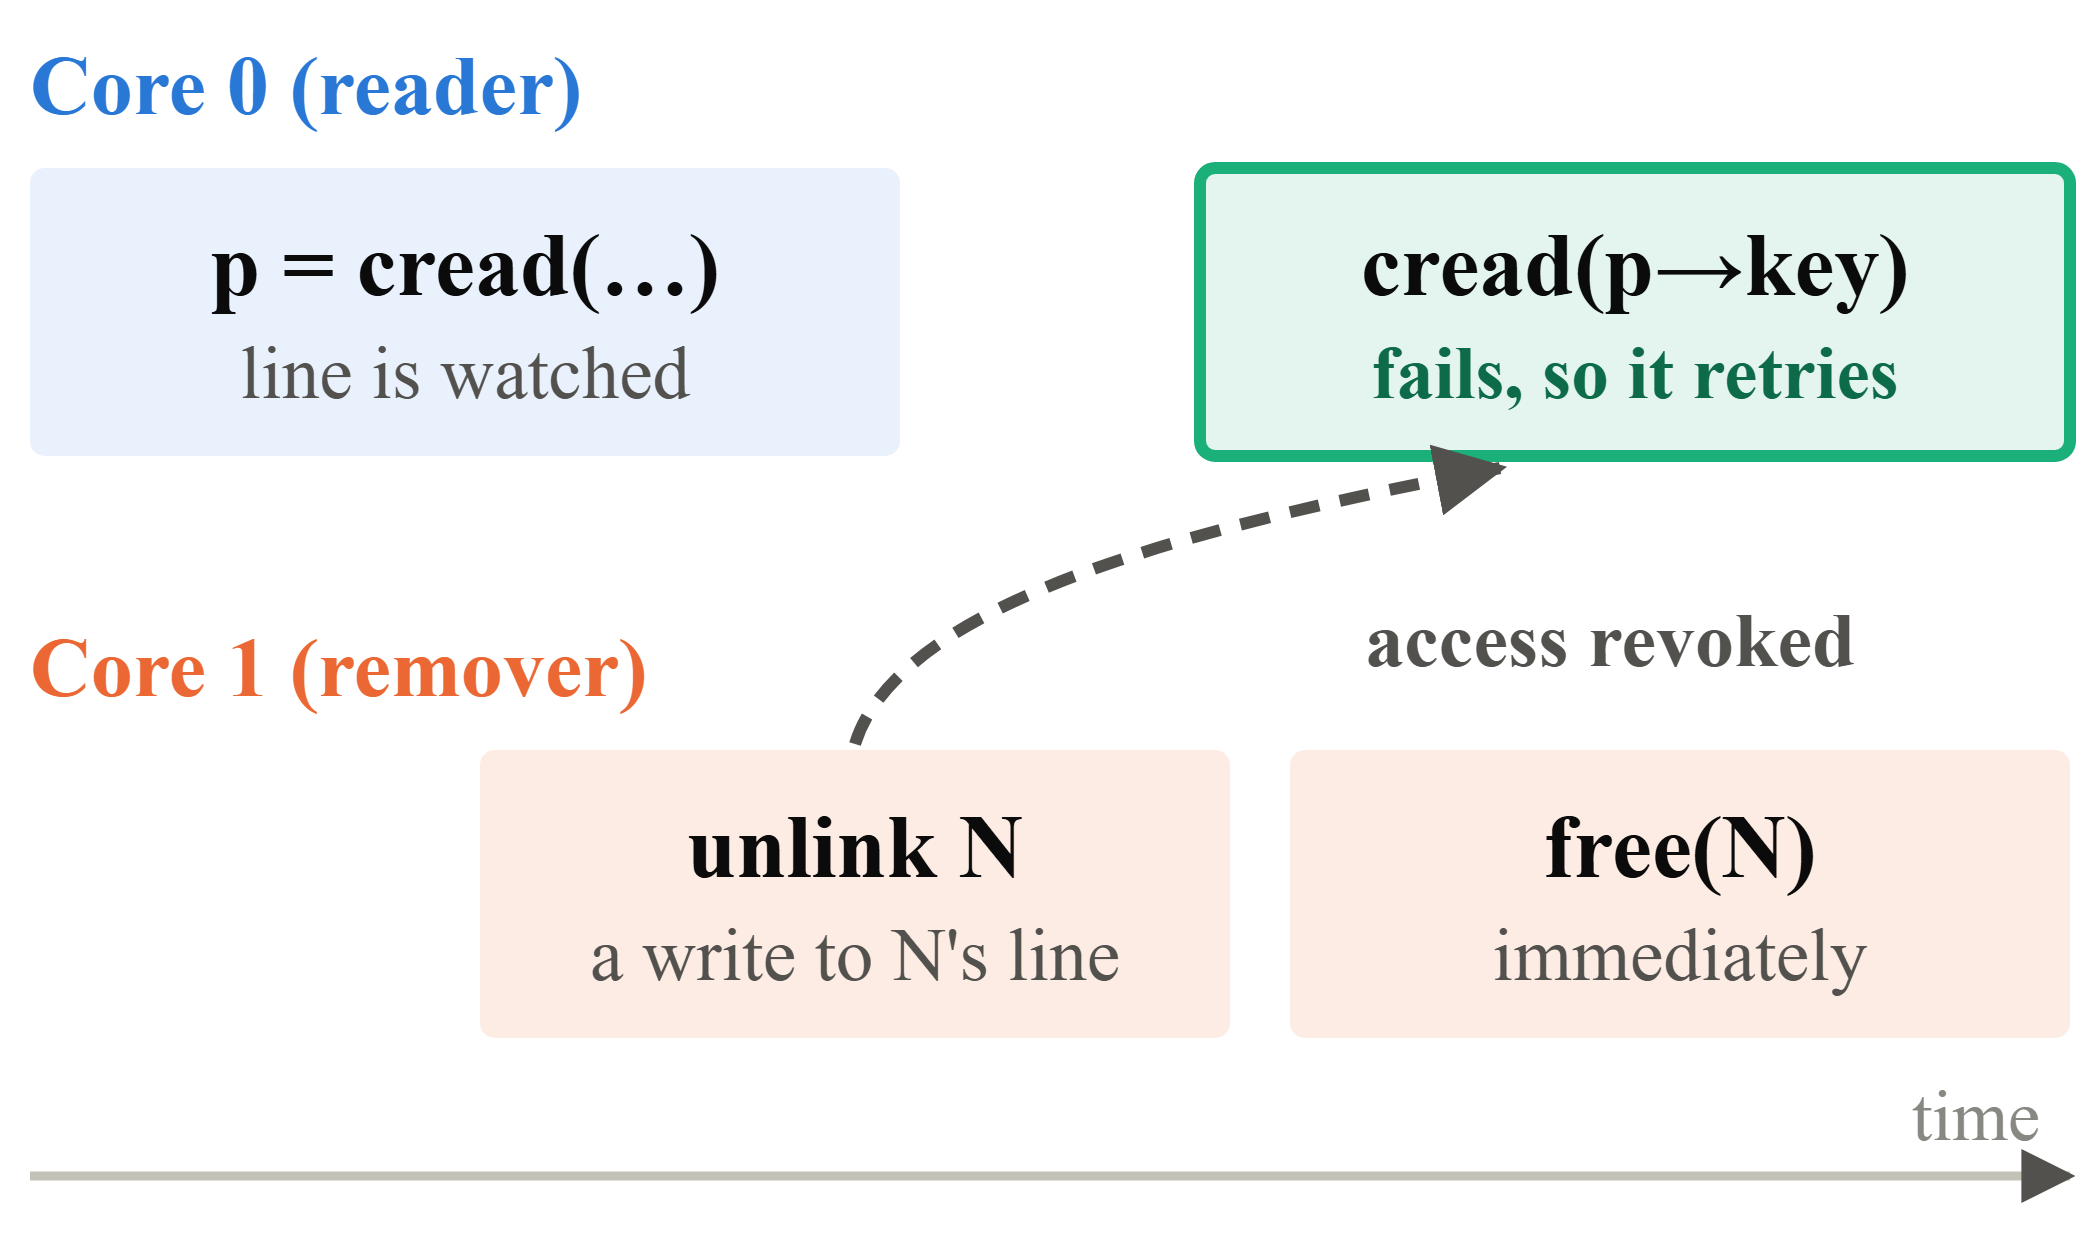
\includegraphics[width=\linewidth]{problem_with.png}
\end{minipage}\hfill
\begin{minipage}[c]{0.53\linewidth}
  \pcaption{With CA, the remover's write revokes the reader's access, so the reader
  retries instead of using freed memory.}
  \vspace{6pt}
  \begin{tabular}{@{}ll@{}}
    \texttt{cread}    & load and watch the line\\
    \texttt{cwrite}   & store if nothing watched changed\\
    \texttt{untagOne} & stop watching one line\\
    \texttt{untagAll} & stop watching all lines\\
  \end{tabular}
\end{minipage}

\vspace{6pt}
\begin{lrbox}{\codebox}
\begin{minipage}{0.97\columnwidth}\codesize
\begin{verbatim}
retry:
  untagAll();
  pred = cread(&head);                 /* read and watch          */
  curr = cread(&pred->next);
  while (cread(&curr->key) < key) {
      if (ca_failed()) goto retry;     /* a watched line changed  */
      pred = curr;  curr = cread(&curr->next);
  }
\end{verbatim}
\end{minipage}
\end{lrbox}
\noindent\fbox{\usebox{\codebox}}\par
{\smallsize\color{captiongray}\textbf{Listing 1.} Searching a lazy list with CA,
simplified from~[1].\par}

%----------------------------------------------------------------------------------------
\psection{Why implement it on an FPGA?}
%----------------------------------------------------------------------------------------
CA was evaluated only on a simulator, which cannot give a high-fidelity picture of its
real performance impact or of the hardware it needs. Implementing it on an FPGA moves CA
from an algorithmic idea to a working hardware mechanism, and tests whether its benefits
survive, or become more compelling, in real hardware. It answers questions a simulator
cannot:
\begin{itemize}
  \item \textbf{Performance:} the real latency of the CA instructions and the throughput
        of data structures that use them (Table~2).
  \item \textbf{Coherence overhead:} what the coherence traffic CA depends on actually
        costs (Table~2).
  \item \textbf{Hardware cost:} the area, logic and memory the mechanism requires (Table~2).
\end{itemize}

%----------------------------------------------------------------------------------------
\psection{System design}
%----------------------------------------------------------------------------------------
We started from CVA6~[2], an open-source single-core RISC-V processor, and added:
\begin{enumerate}[label=(\arabic*),leftmargin=2.2em]
  \item a second core with its own private data cache;
  \item MSI cache coherence between the two caches, which CA relies on;
  \item the four CA instructions in the processor pipeline.
\end{enumerate}

\posterfig[\figscale]{architecture.png}{The two-core system on the AMD KR260. Blocks
marked \emph{new} were designed in this work.}

Each cache line is Modified, Shared or Invalid. A cache takes the shared bus before
touching memory and the other cache writes back dirty data first, so memory stays current
and no L2 is needed. Programs run bare metal: the host loads them over JTAG and reads
results from an uncached mailbox.

\columnbreak

%----------------------------------------------------------------------------------------
\psection{Challenges}
%----------------------------------------------------------------------------------------
\textbf{Choosing a base.} We first tried OpenPiton, the usual route to a multicore CVA6.
It is a heavy framework built around an older CVA6: we would have had to bring it up to
date with current CVA6 before adding our changes, including a new L1.5 adapter. We
dropped it and built a coherent two-core system directly on current CVA6.

\textbf{Fitting the FPGA.} The KR260's limited LUTs made it hard to fit a two-core 64-bit
system with room for our tests, so we moved to the 32-bit (RV32) CVA6 and designed the caches,
coherence and tests around it. The final system uses 50\% of the LUTs and 51\% of the
block RAM, and meets timing at 50\,MHz; each CA unit tracks 8 lines.

\textbf{Deadlock freedom.} A cache can always answer the other cache's coherence request
without needing the shared bus itself, so one of the two always makes progress.

\textbf{Atomic \texttt{cwrite}.} The check and the store must be indivisible.
\texttt{cwrite} waits until it is the oldest instruction and holds the cache line
exclusively, so no other core can write between the check and the store.

\textbf{Speculation.} The pipeline issues instructions before it knows they will
complete. CA operations are recorded at issue and take effect only at commit, so a
cancelled instruction leaves no trace.

\textbf{Learning curve.} We had to learn CVA6's microarchitecture, the KR260 and its
Vivado flow, and the underlying concepts: cache coherence, RISC-V atomics and lock-free
memory reclamation.

%----------------------------------------------------------------------------------------
\psection{Verification}
%----------------------------------------------------------------------------------------
We verified at three levels: Verilator testbenches for one and two caches driven by
random traffic, the full processor running standard RISC-V test suites, and two-core
programs on the board.
\begin{itemize}
  \item 1,100 of 1,100 randomized simulations pass against models of MSI and of CA~[1].
  \item 26 of 27 deliberately injected bugs are detected; the remaining mutant cannot
        change behaviour with two caches.
  \item 72 of 73 RISC-V ISA tests pass in simulation and on the FPGA, and the two-core
        coherence and CA programs pass 20 of 20 board runs.
  \item The testbenches found two real races in our first design (a stale shared copy
        during an upgrade, and an LR/SC livelock between the cores), both fixed.
\end{itemize}
Negative control: with ordinary loads the board program reads freed memory; with
\texttt{cread} it never does.

%----------------------------------------------------------------------------------------
\psection{Evaluation}
%----------------------------------------------------------------------------------------
We ran the benchmarks of~[1] (lazy list, external BST, Treiber stack, hash table) on both
cores at 50\,MHz, bare metal, with 3,000 operations per thread, 0, 10 and 100\% updates
and 3 seeds: 288 runs, each followed by a check of the data structure. Table~1 compares
our platform with the paper's.

\vspace{4pt}
{\centering
{\smallsize\color{captiongray}\textbf{Table 1.} Evaluation platform: the paper and this work.\par}
\vspace{3pt}
{\smallsize
\begin{tabular}{lll}
\toprule
 & Singh et al.~[1] & This work\\
\midrule
Platform & Graphite simulator & AMD KR260 FPGA, 50\,MHz\\
Cores & 1 to 32 & 2 (CVA6, RV32)\\
Coherence & directory MSI & snooping MSI on a shared bus\\
Cache line, L2 & 64\,B, 256\,KiB shared L2 & 16\,B, no L2\\
\bottomrule
\end{tabular}\par}}

\posterfig[0.85]{throughput.png}{Throughput relative to never freeing memory (higher is better),
two cores. Bars above the dashed line outperform the leaking baseline.}

\posterfig[0.65]{unfreed.png}{Nodes removed but not yet freed at the end of a run,
averaged over the four data structures (two cores, 100\% updates).}

\begin{itemize}
  \item Under the highest contention, CA is the fastest scheme: 1.33$\times$ the leaking
        baseline on the stack, against 1.09$\times$ for hazard pointers and 1.05$\times$
        for epochs.
  \item From 1 to 2 threads on that stack, the leaking baseline falls from 0.36 to
        0.19\,Mops/s, while CA goes from 0.40 to 0.25 and stays ahead.
  \item CA frees every node immediately; the other schemes leave tens to thousands of
        nodes waiting.
  \item In read-mostly workloads CA is slower, as in~[1]: the cost is the failure check
        (a status-register read at commit), not \texttt{cread} itself (Table~2).
\end{itemize}

\vspace{4pt}
{\centering
{\smallsize\color{captiongray}\textbf{Table 2.} What the FPGA measured: answers to the questions in Section~4.\par}
\vspace{3pt}
{\smallsize
\begin{tabular}{@{}p{0.2\columnwidth}p{0.77\columnwidth}@{}}
\toprule
Question & Measured on the KR260\\
\midrule
Latency & load 1 cycle; \texttt{cread} 2; \texttt{cread} + failure check 7;
  \texttt{cread} + \texttt{cwrite} 17 (\texttt{amoswap} 14; hazard-pointer fence 6)\\
Throughput & up to 1.33$\times$ the leaking baseline under contention (Figure~4);
  0 nodes left unfreed (Figure~5)\\
Coherence overhead & read miss 54 cycles, 97 if the other core holds the line dirty;
  invalidating a clean remote copy adds about 1 cycle; core-to-core handoff 151 cycles\\
Area, logic, memory & CA unit 1,139 LUTs + 538 flip-flops per core (4.5\% of a core,
  1\% of the FPGA), no block RAM; coherence bus 48 LUTs + 40 flip-flops\\
\bottomrule
\end{tabular}\par}}

%----------------------------------------------------------------------------------------
\psection{Conclusions}
%----------------------------------------------------------------------------------------
We built and verified a dual-core RISC-V processor with Conditional Access and the cache
coherence it depends on, running on an FPGA. It reclaims memory immediately and is the
fastest scheme under contention, confirming the findings of~[1] on real hardware.
Future work: a branch-on-failure instruction to make the check cheap, and more cores with a scalable interconnect.

\vspace{4pt}
{\smallsize
\textbf{References.}
[1] A.~Singh, T.~Brown, M.~Spear. Efficient hardware primitives for immediate memory
reclamation in optimistic data structures. arXiv:2302.12958, 2023.
[2] F.~Zaruba, L.~Benini. The cost of application-class processing. \emph{IEEE TVLSI}, 2019.
[3] M.~M.~Michael. Hazard pointers: safe memory reclamation for lock-free objects.
\emph{IEEE TPDS}, 2004.
[4] T.~E.~Hart et al. Performance of memory reclamation for lockless synchronization.
\emph{JPDC}, 2007.\par\vspace{3pt}
\textbf{Acknowledgements.} We thank Prof.\ Ajay Singh for his guidance throughout this
project, and the Department of Computer Science and Engineering, IIT Gandhinagar, for
access to the AMD KR260 board and tools.\par}

\end{multicols}
\end{document}
